\subsection{研究背景}
近年,深層学習は大きな発展を見せている.
Recurrent Neural Network\cite{rnn}はConvolutional Neural Network\cite{cnn}にはない
「時間」という概念を持ち,機械翻訳の分野で大きな成果を出した.
一方で,小説などの大きな入力には対応できないという欠点もあった.
RNNに長期的記憶の概念を導入したLSTM\cite{lstm}やGRU\cite{gru}も開発されたが,
計算時間の増加が問題であった.

2017年に登場したTransformer\cite{transformer}は単純な行列計算のみで完結したネットワークで,
機械翻訳でこれまでのRNNを超える精度を出し,計算時間も大幅に削減したことで,
機械翻訳のデファクトスタンダードとなった.
2020年にはVision Transformer\cite{vit}が開発され,画像認識でCNNを超える精度を出した.
さらに翌年にはVideo Vision Transformer\cite{vivit}が開発され,動画解析でもRNNを超える精度を出した.

AIの活躍は単純なタスクに留まらない.ボードゲームでは,
囲碁のAlphaGo\cite{alphago},その後継でフレームワークとして
開発されたAlphaZero\cite{alphazero}は囲碁,チェス,将棋で成果を上げている.
芸術ではMusic Transformer\cite{mut}で作曲,DALL-E2\cite{dalle2}で作画が可能となっている.

「優美さ」とは,人間の動作を表現する形容詞である.Buytendijkは,優美な動作とは
\begin{enumerate}
  \item ゆっくりとした,丸みのある動き
  \item 持続性と流動性を持つ動き
  \item 緊張と解繁がリズミカルに交替して現れる動き
\end{enumerate}
であると主張した.
またHogarthは,図\ref{hogarth_curve}のような「美の線」を多く含むものであると主張した.

Transformerにより更に応用の幅が広がったAIで優美さを評価した場合,先人たちの見ていた視点とは
違った視点を見ることができると考え,本研究に至った.

\begin{figure}[b]
  \begin{center}
   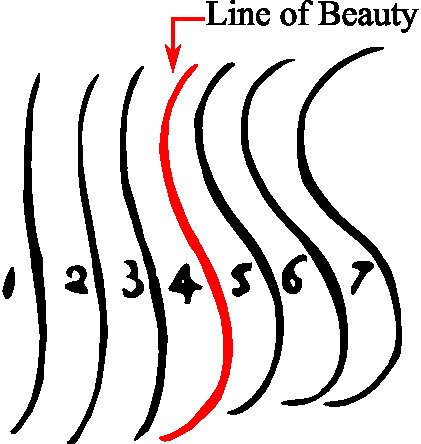
\includegraphics[width=40mm]{images/hogarth_curve.pdf}
  \end{center}
  \caption{Hogarth Curve}
  \label{hogarth_curve}
\end{figure}

\clearpage

\subsection{研究目的}
本研究では,深層学習を用いて上田研のテーマとする「優美さ」を対象に,
より網羅的に検証した場合の結果を得て,それを先行研究らと比較することを目的とする.

我々の研究室ではHogarthの規範に則り,動作解析や動作生成を行ってきた.
稲津\cite{inadu}は手先の軌道をB-spline近似\cite{bspline}したのちに
\begin{enumerate}
  \item 軌道長がより長い
  \item Hogarth Curveとの形状類似度
  \item 両弧の弧長がほぼ等しい
  \item 両弧の全曲率が0.873〜1.44
\end{enumerate}
を検証する評価モデルを提案した.

照岡\cite{teruoka}は強化学習を用いて曲線の生成を試みた.シミュレータ上で駆動する
仮想ロボットアームを,強化学習から生成される動作で動かした.
目標点との位置差分と各関節の加速度を用いて,照岡の提案する様々な報酬関数でで学習を進めた.
それらの動作を同じくB-spline近似し,先の稲津の評価モデルで優美さを検証した.

これらの研究は手先軌道に限定して着目したもので,論文内でも他部位との関係検証の必要性や
特定状況下でしか機能しないことが言及されている.
実際,上田研では実データとして既存のcsvデータを使用するにとどまっていた.
さらに最終的な優美評価はアンケートによる主観評価で,これもデータ量として少ないものであった.

深層学習を用いることでデータに依存しないネットワーク構築が可能であり,
データが増えるほど精度が上がることが期待できる.
さらに,mp4を実データとすることでデータ収集も容易かつ大量に行うことが可能となった.
動画全体を対象とすることで目的とする網羅的検証も可能となり,これにより
従来の解析手法との比較から得られる相違点,共通点が明瞭となると考える.

\subsection{研究概要}